\chapter{Spanning Tree Protocol}

\section{Switch Manual}
The user manual for the switch is available here:


\ifpdf
\url{http://www.jaumebarcelo.info/teaching/lxs/stp/manual_spantree.pdf}
\else
\texttt{http://www.jaumebarcelo.info/teaching/lxs/stp/manual\_spantree.pdf}
\fi


\section{Introduction}

In this assignment you will configure the Spanning Tree Protocol.
This protocol is used in Ethernet networks to establish which are the active link and therefore which is the path that data packets will follow.
The switches that you will use are the same as the ones in the previous assignment.
Have your VLAN report handy just in case you need to consult it to refresh which are the basic commands to interact with the switch.

\section{Theoretical construction of the tree}
The switches are connected as depicted in Fig. \ref{fig:stp_topology}.
\begin{figure}[htbp]
  \centering
  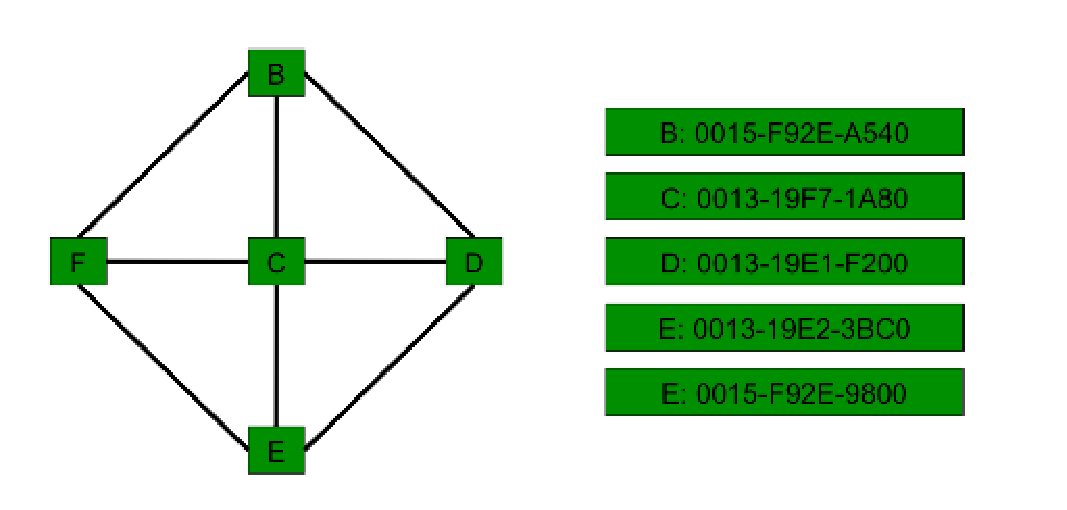
\includegraphics[width=0.4\linewidth]{figures/stp_topology.eps}
  \caption{Network topology}
  \label{fig:stp_topology}
\end{figure}

Find the BridgeId of each switch.
Compute which is the spanning tree and draw it.
Which switch is the root?
Which is the role of each port?
Which ports are activated?

\section{Practical verification}

Now you will verify that the STP constructed by the switches is in fact the one you computed in the previous section.

Use the VLAN 1 to connect to the five switches (B, C, D, E, F).
It is recommended to open five windows and telnet one of the switches in each of them.

Each group will work in a different VLAN.
The teacher will assign a VLAN to each group.
Make sure that your VLAN is included in all the trunk ports.
Each group will have a different STP, as the network creates a tree for each VLAN.

In each of the switches, enter the privileged EXEC mode and use the command \texttt{show spanning-tree vlan XX}.
What can you see?
Observe all the fields and make sure you understand them.

Find the BridgeId of each switch.
Compute which is the spanning tree and draw it.
Which switch is the root?
Which is the role of each port?
Which ports are activated?


